\subsection[Ridurre la Loss]{Ridurre la Loss}

\subsubsection[Un approccio iterativo]{Un approccio iterativo}
\begin{frame}

	\frametitle{Un approccio iterativo alla riduzione della Loss}

	%\begin{block}{}
		L'apprendimento iterativo potrebbe ricordare il gioco per bambini ``\textit{Acqua, fuochino, fuoco...}'' per trovare un oggetto nascosto nella stanza.
		\newlinedouble
		In questo gioco, l '\textbf{oggetto nascosto} è il \textbf{miglior modello} possibile.
		\newline
		Solitamente si parte con un'ipotesi folle (nel nostro contesto inizializzando il valore di $\omega_1$ a $0$ ad esempio) e attendi che il \textit{sistema} ti dica qual è il valore della Loss.
		\newlinedouble
		Quindi, si prova un'altra ipotesi (ad es: il valore di $\omega_1$ è $0.5$) e si valuta qual è la nuova loss.
		Aah! Sta diventando più caldo!
		\newlinedouble
		In realtà, se si gioca bene a questo gioco, di solito ci si scalda.\\
		Il vero trucco del gioco sta nel provare a trovare il \textbf{miglior modello} possibile \textbf{nel modo più efficiente} possibile.
	%\end{block}

\end{frame}


\begin{frame}

	\frametitle{Un approccio iterativo alla riduzione della Loss}

	%\begin{block}{}
		Le strategie iterative sono le più utilizzate nell'apprendimento automatico, principalmente perché si adattano molto bene a datasets di grandi dimensioni.\\
		La figura mostrata mostra il processo iterativo per tentativi ed errori (\textbf{trial-and-error}) utilizzato dagli algoritmi di apprendimento automatico per addestrare un modello:

		\begin{figure}[!htbp]
			\centering
			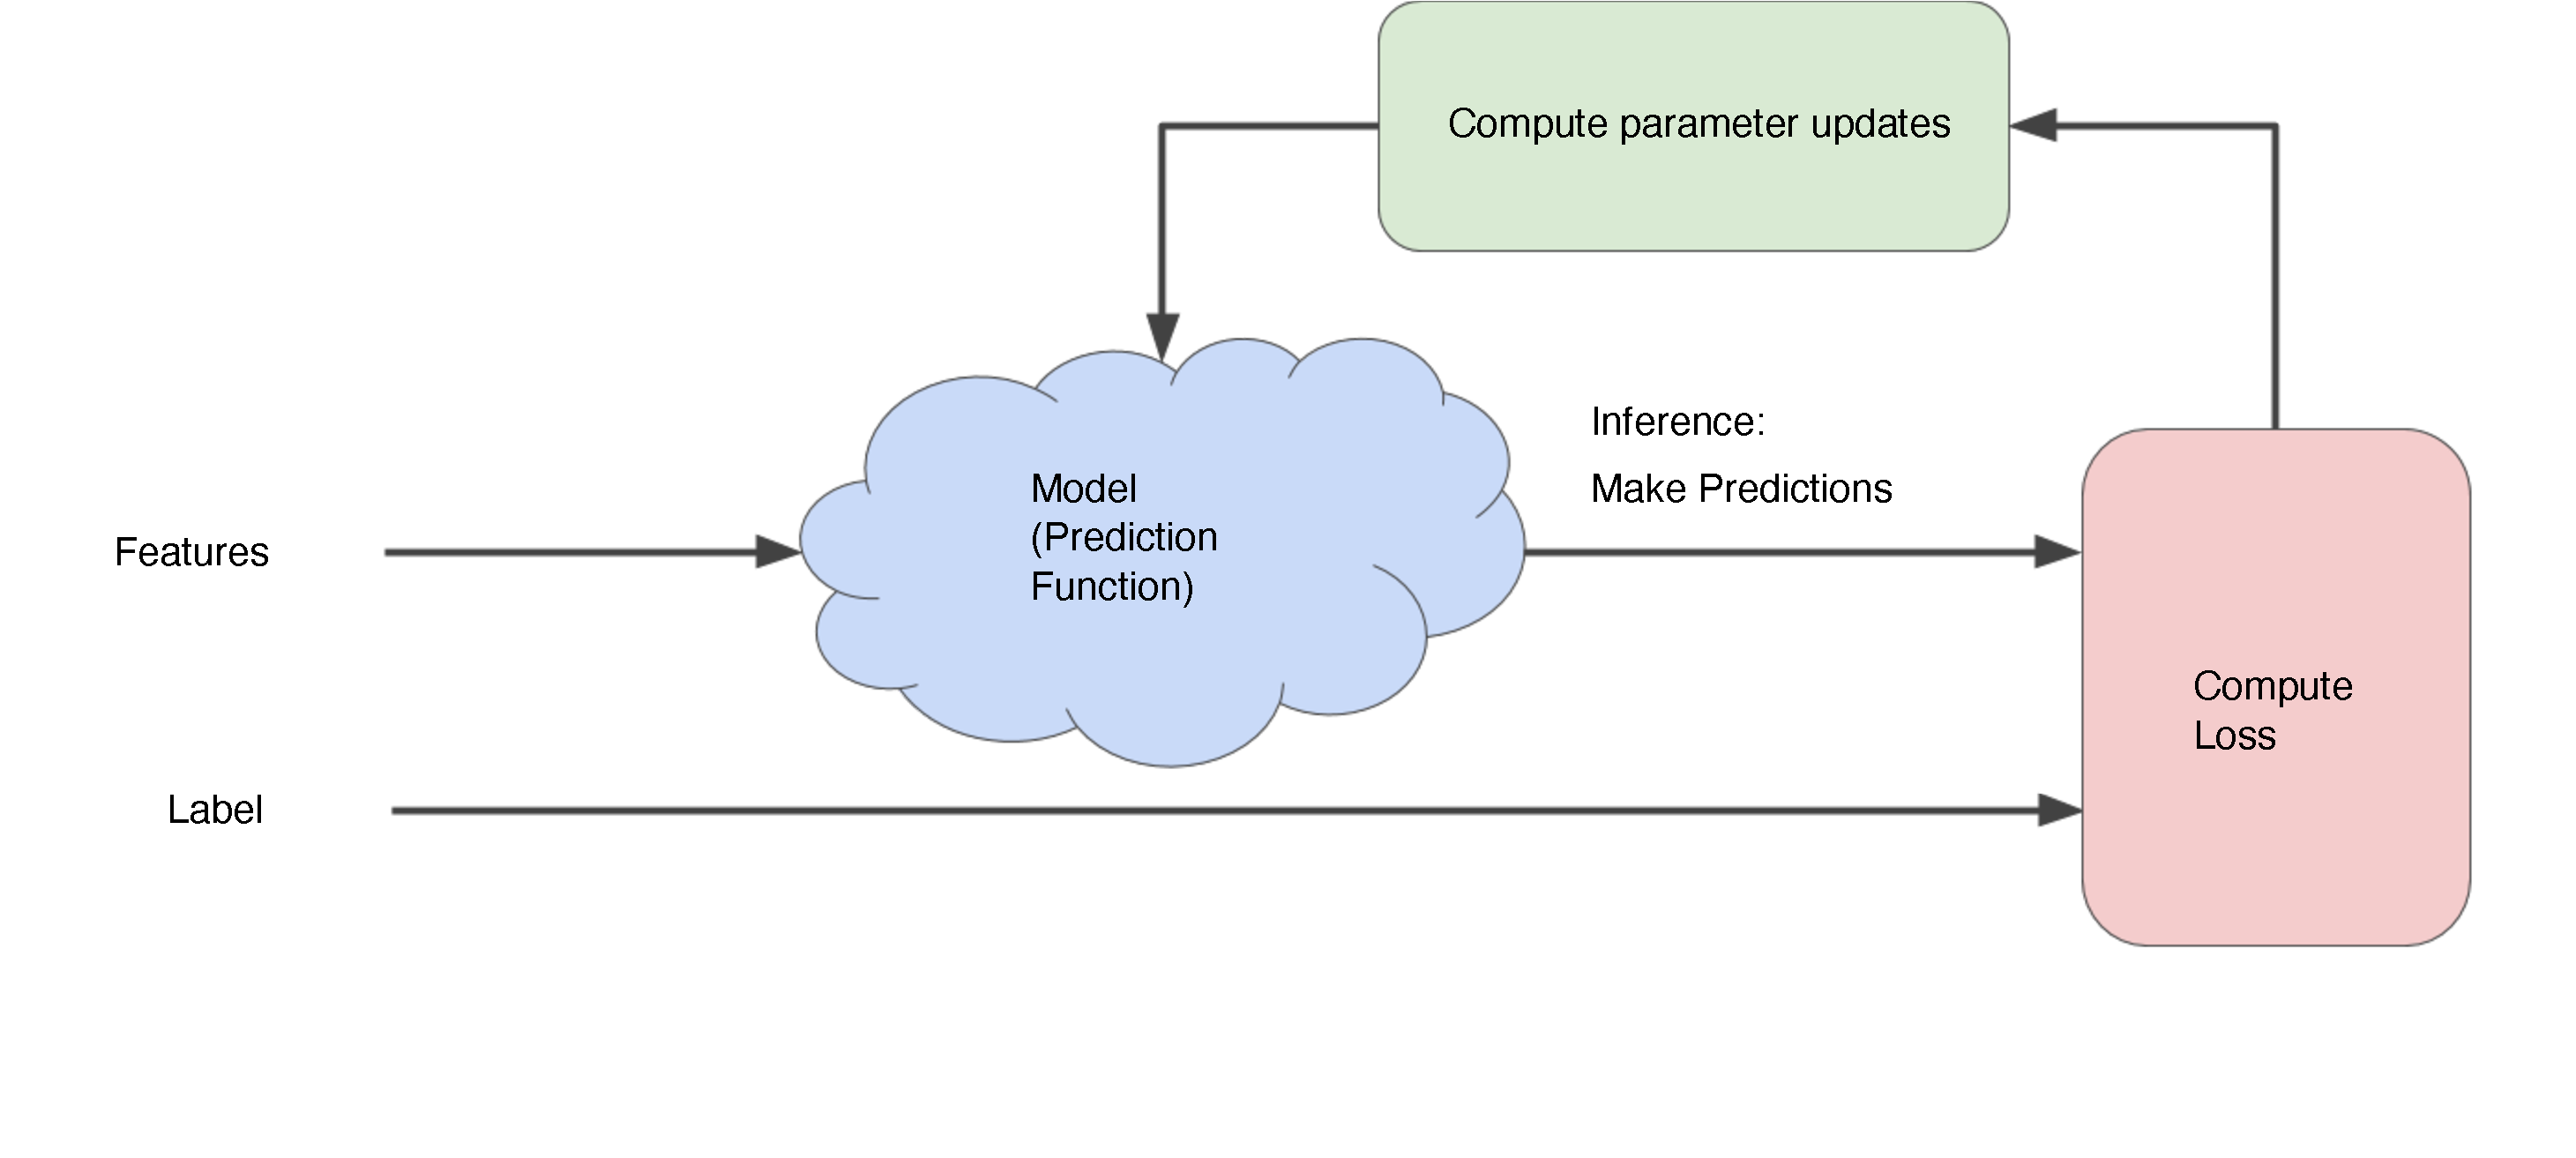
\includegraphics[width=0.8\linewidth]{images/supervised/training_reducing_loss/GradientDescentDiagram.pdf}
			%\caption{Stripe Radar for Fraud Detection}
			\end{figure}

	%\end{block}

\end{frame}



\begin{frame}

	\frametitle{Un approccio iterativo: {\color{GradientDescentDiagramBlue}``Model (Prediction Function)''}}

	%\begin{block}{Iterative approach: Model (Prediction Function)}
		Il ``modello'' accetta una o più features come input e restituisce una previsione ($y'$) come output.\\
		Per semplificare, consideriamo un modello che accetta una feature e restituisce una previsione:
		$$y' = b + \omega_1x_1$$

		Quali valori iniziali dovremmo impostare per $b$ e $\omega_1$?\\
		Per i problemi di regressione lineare in realtà la modalità con cui scegliamo i valori iniziali non è così importante.\\
		Potremmo scegliere valori casuali, ma prenderemo invece i seguenti valori:
		$$b = 0 \quad \omega_1 = 0$$

		Fissati i due parametri ho una prima versione di un possibile modello.
		$$\forall x_1: \quad y' = 0 + 0x_1 = 0$$
	%\end{block}

\end{frame}


\begin{frame}

	\frametitle{Un approccio iterativo: {\color{GradientDescentDiagramRed}``Compute Loss''}}

	%\begin{block}{Iterative approach: Compute Loss}
		La parte \textbf{Compute Loss} del diagramma è la funzione di loss che il modello utilizzerà.
		\newlinedouble
		Supponiamo di utilizzare la $L_2$.\\
		Questa loss, come abbiamo visto, accetta due valori di input:
		\begin{itemize}
			\item $y'$: la previsione del modello per le caratteristiche x
			\item $y$: l'etichetta corretta corrispondente alle caratteristiche x
		\end{itemize}

		\vspace{4mm}
		Potremmo calcolare la loss $L_2$ su tutti gli esempi nel seguente modo:
		$$L_2(model, \mathcal{D}) = \sum_{(x,y)\in\mathcal{D}} \left( y-prediction_{model}(x) \right)^2 = \sum_{(x,y)\in\mathcal{D}}(y-y')^2$$

	%\end{block}

\end{frame}


\begin{frame}

	\frametitle{Un approccio iterativo: {\color{GradientDescentDiagramGreen}``Compute parameter updates''}}

	%\begin{block}{Iterative approach: Compute parameter updates}

		Siamo arrivati quindi alla sezione \textbf{Compute parameter updates}.\\
		È qui che il sistema di apprendimento automatico esamina il valore della loss e genera nuovi valori per $b$ e $\omega_1$.
		\newlinedouble
		Per ora, supponi che questa sia una \textbf{scatola nera} elabori nuovi valori e quindi il sistema di apprendimento automatico rivaluti tutte quelle feature rispetto a tutte quelle lables, producendo un nuovo valore per la funzione di loss, che porta ad aggiornare i parametri con nuovi valori.
		\newlinedouble
		E l'apprendimento continua fino a quando l'algoritmo scopre i parametri del modello con la minima perdita possibile.\\
		Di solito, \textbf{si itera fino a quando la perdita complessiva non smette di cambiare o almeno cambia estremamente lentamente}.\\
		Quando ciò accade, diciamo che il modello \textbf{converge}.

	%\end{block}

\end{frame}


\begin{frame}

	\frametitle{Un approccio iterativo alla riduzione della Loss}

	\begin{block}{Ricapitolando}
		Un modello di Machine Learning viene addestrato partendo da un'ipotesi iniziale per pesi e bias e regolando in modo iterativo tali ipotesi fino ad apprendere pesi e bias con la loss più bassa possibile.
		\begin{figure}[!htbp]
			\centering
			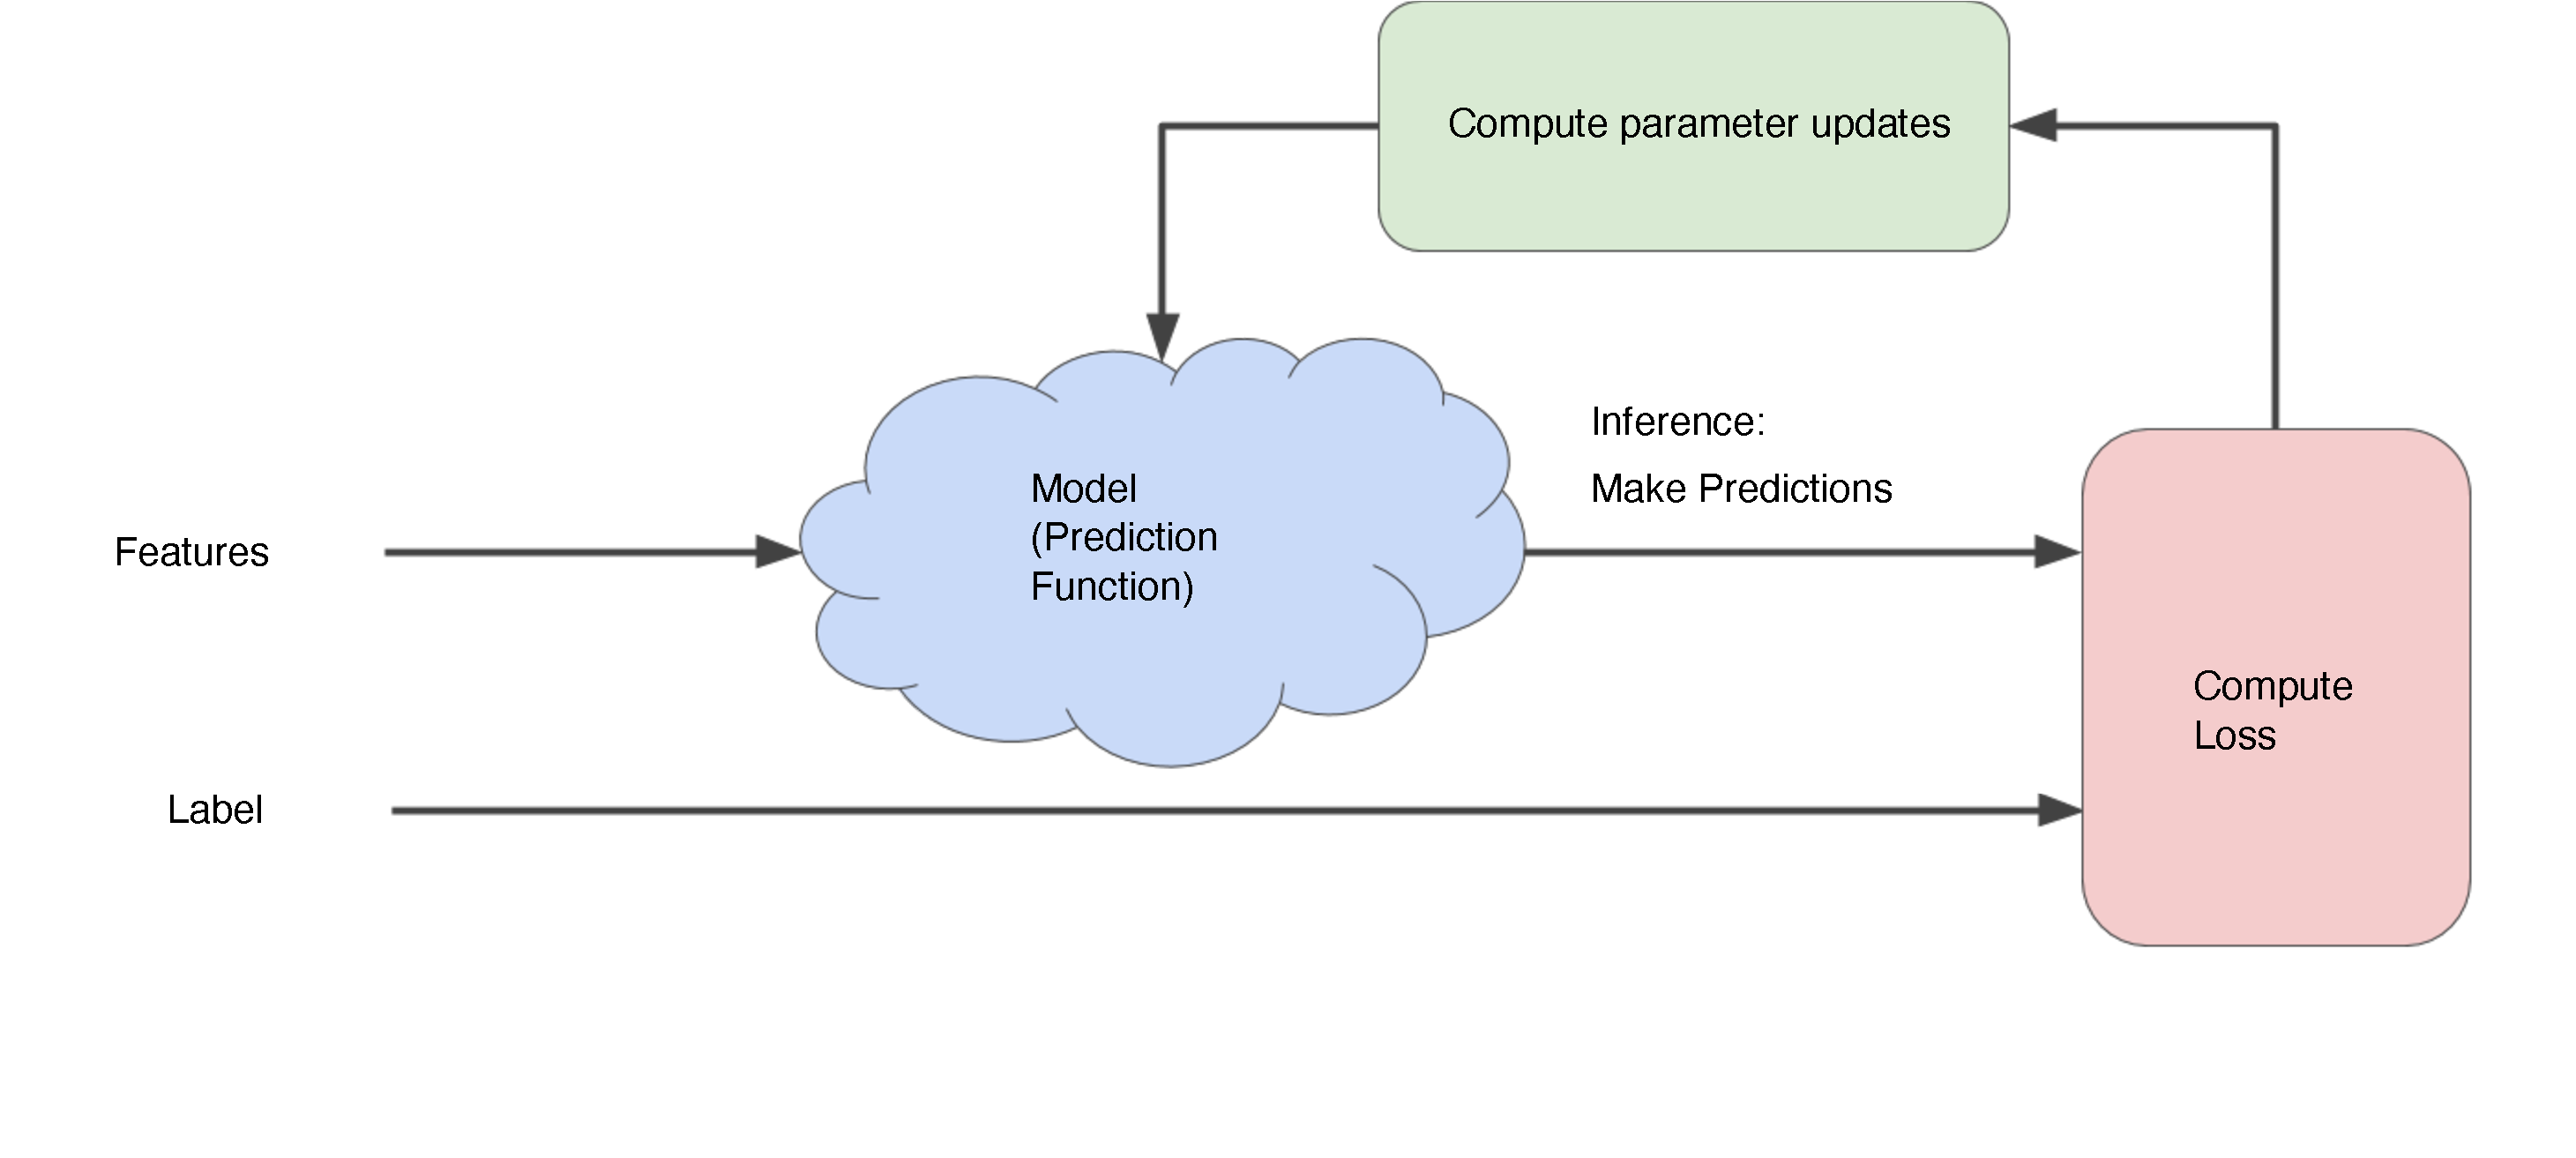
\includegraphics[width=0.9\linewidth]{images/supervised/training_reducing_loss/GradientDescentDiagram.pdf}
			%\caption{Stripe Radar for Fraud Detection}
		\end{figure}

	\end{block}

\end{frame}



\subsubsection[La discesa del gradiente (GD)]{La discesa del gradiente (GD)}
\begin{frame}

	%\frametitle{La discesa del gradiente:\\come strategia per il {\color{GradientDescentDiagramGreen}``Compute parameter updates''}}
	\frametitle{La discesa del gradiente}

	\begin{block}{La discesa del gradiente: strategia per il {\color{GradientDescentDiagramGreen}``Compute parameter updates''}}
		Supponiamo di avere il tempo e le risorse di calcolo per calcolare la loss per tutti i possibili valori di $\omega_1$.\\
		Per il tipo di problemi di regressione che abbiamo esaminato, il grafico risultante della loss rispetto a $\omega_1$ sarà sempre \textbf{convesso}.\\
		\vspace{3mm}
		In altre parole, il grafico risultante $\omega_1 \rightarrow loss$ sarà sempre a forma di ciotola, un po' come nella seguente immagine:
		\begin{figure}[!htbp]
			\centering
			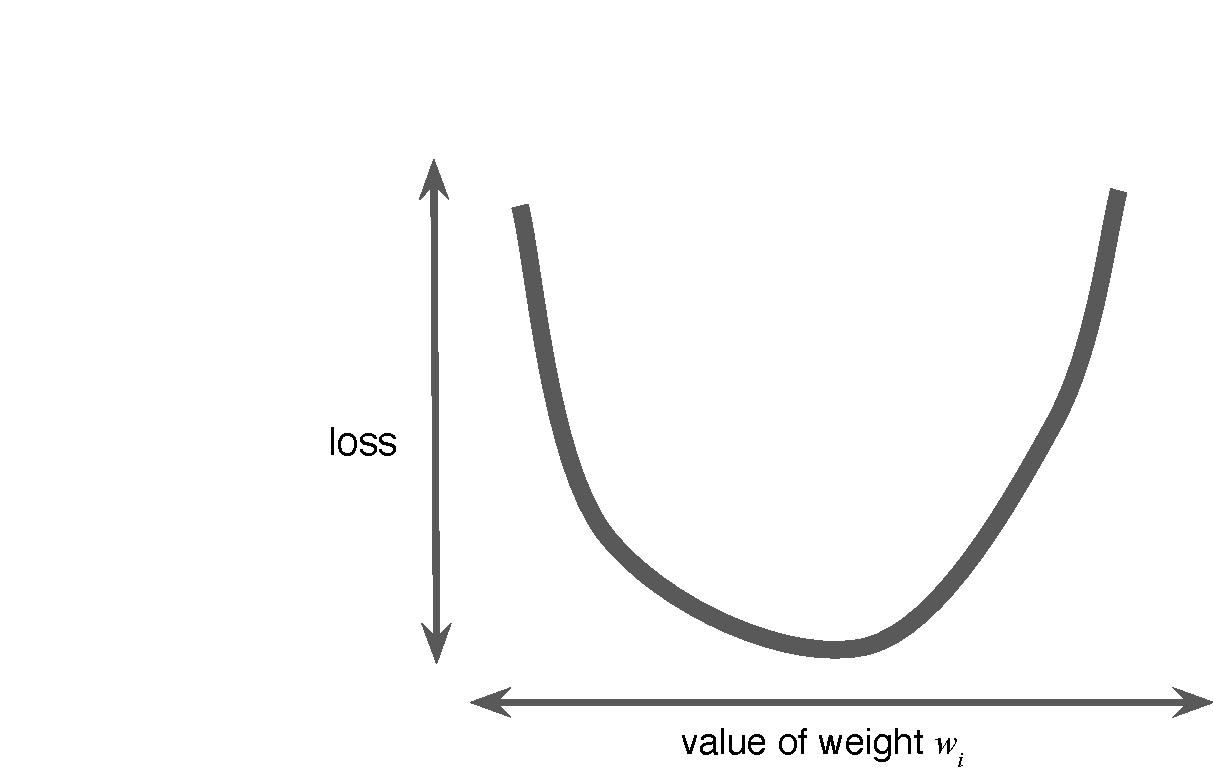
\includegraphics[width=0.35\linewidth]{images/supervised/training_reducing_loss/convex.pdf}
			%\caption{Stripe Radar for Fraud Detection}
		\end{figure}

	\end{block}

\end{frame}


\begin{frame}

	\frametitle{La discesa del gradiente: osservazioni}

	\begin{block}{Osservazioni}

		\begin{itemize}
			\item i problemi convessi hanno solo un minimo; cioè, solo un punto in cui la pendenza è esattamente 0
			\item quel minimo corrisponde a dove la loss converge
			\item calcolare la loss per ogni valore concepibile di $\omega_1$ sull'intero dataset sarebbe un modo inefficiente per trovare il punto di convergenza
		\end{itemize}

		Esaminiamo un meccanismo migliore, molto popolare nell'apprendimento automatico, chiamato \textbf{discesa del gradiente}.

	\end{block}

\end{frame}


\begin{frame}

	\frametitle{La discesa del gradiente}

	\begin{block}{L'agoritmo di discesa del gradiente (GD): la scelta del valore iniziale}
		La prima fase nella discesa del gradiente consiste nello \textbf{scegliere un valore iniziale} (un punto di partenza) per $\omega_1$.\\
		Il punto di partenza non ha molta importanza; pertanto, molti algoritmi impostano semplicemente $\omega_1$ su 0 o scelgono un valore casuale.\\
		\vspace{1mm}
		Nella figura abbiamo scelto un punto di partenza leggermente $>0$:
		\begin{figure}[!htbp]
			\centering
			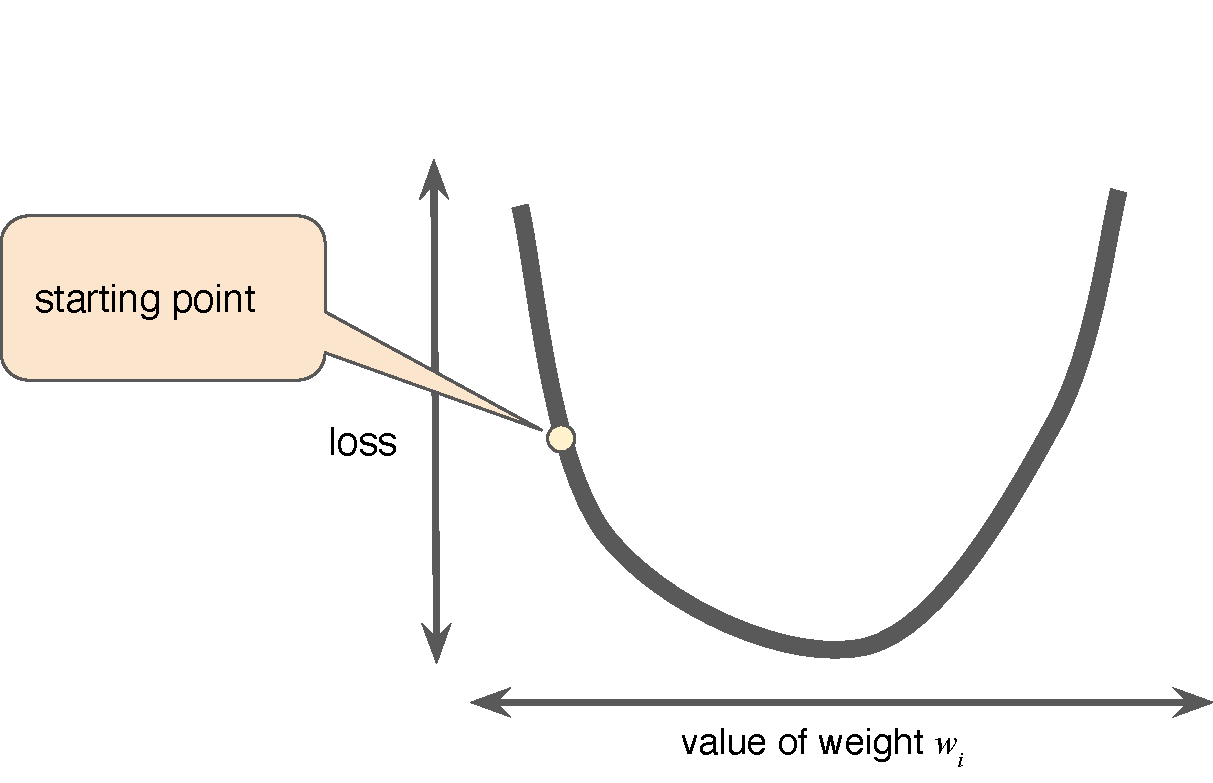
\includegraphics[width=0.55\linewidth]{images/supervised/training_reducing_loss/GradientDescentStartingPoint.pdf}
			%\caption{Stripe Radar for Fraud Detection}
		\end{figure}
	\end{block}

\end{frame}


\begin{frame}

	\frametitle{La discesa del gradiente}

	\begin{block}{L'agoritmo di discesa del gradiente (GD): l'aggiornamento di $\omega_1$}
		Il GD calcola quindi il gradiente della curva della loss nel punto iniziale.\\
		Nella figura il gradiente della loss è uguale alla derivata (pendenza) della curva e ti dice in quale direzione è ``più caldo'' o ``più freddo''.\\
		\vspace{1mm}
		Quando ci sono più pesi ($b$, $\omega_1$, $\omega_2$, etc), il gradiente è un vettore di derivate parziali rispetto ai pesi.

		\begin{figure}[!htbp]
			\centering
			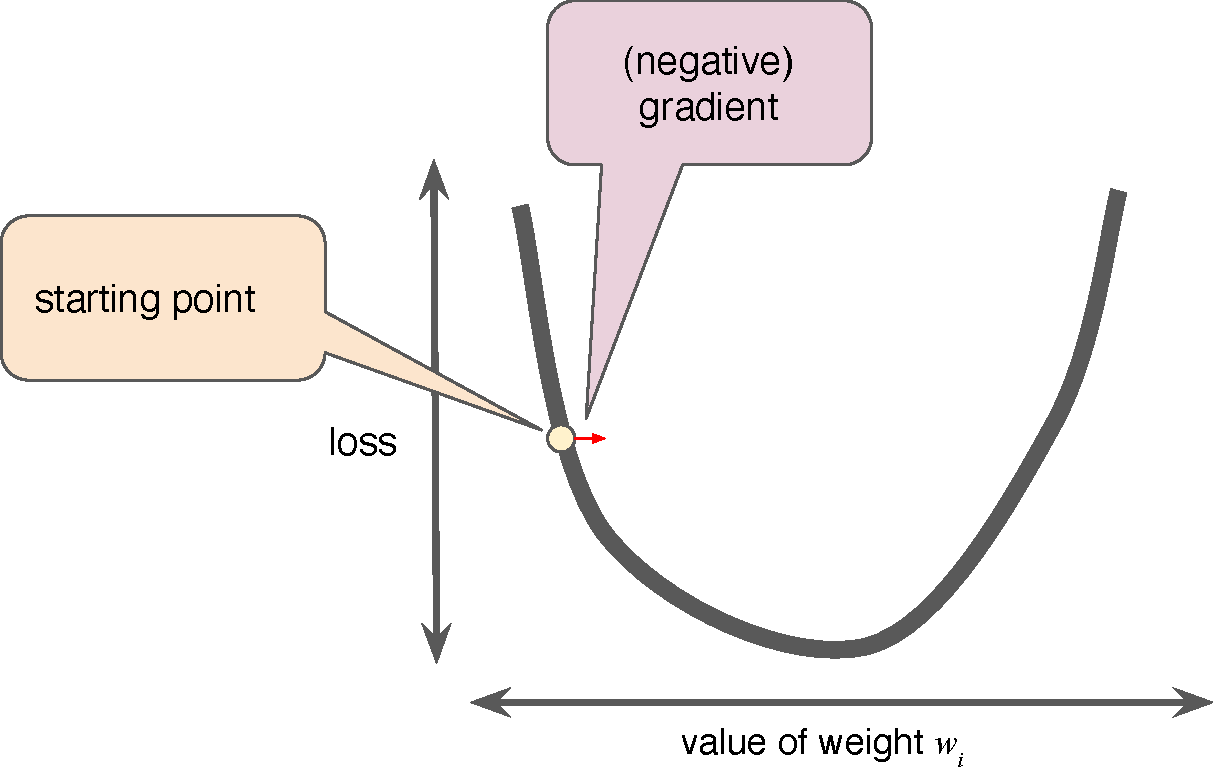
\includegraphics[width=0.45\linewidth]{images/supervised/training_reducing_loss/GradientDescentNegativeGradient.pdf}
			%\caption{Stripe Radar for Fraud Detection}
		\end{figure}
	\end{block}

\end{frame}


\begin{frame}

	\frametitle{Il gradiente}

	%\begin{block}{}
		Il gradiente di una funzione, indicato come segue, è il 	\textbf{vettore delle derivate parziali} rispetto a tutte le variabili indipendenti:

		$$\nabla f$$

		Ad esempio se:
		$$f(x, y) = e^{2y}sin(x)$$

		allora:

		$$\nabla f(x, y)= \left( \frac{\partial f}{\partial x} (x, y), \frac{\partial f}{\partial y} (x, y)\right) = \left(e^{2y}cos(x), 2e^{2y}sin(x)\right)$$

		Si noti che:
		\begin{itemize}
			\item $+\nabla f$ indica sempre la direzione del maggior incremento della funzione
			\item $-\nabla f$ indica sempre la direzione di maggiore diminuzione della funzione
		\end{itemize}
	%\end{block}

\end{frame}


\begin{frame}

	\frametitle{La discesa del gradiente}

	%\begin{block}{}
		Si noti che il gradiente è un vettore, quindi ha le seguenti caratteristiche:
		\begin{itemize}
			\item una direzione e un verso
			\item un'intensità
		\end{itemize}

		Il gradiente punta sempre nella direzione di aumento più ripido della loss.\\
		L'algoritmo di discesa del gradiente fa uno step nella direzione di $-\nabla f$ per ridurre la loss il più rapidamente possibile.

		\begin{figure}[!htbp]
			\centering
			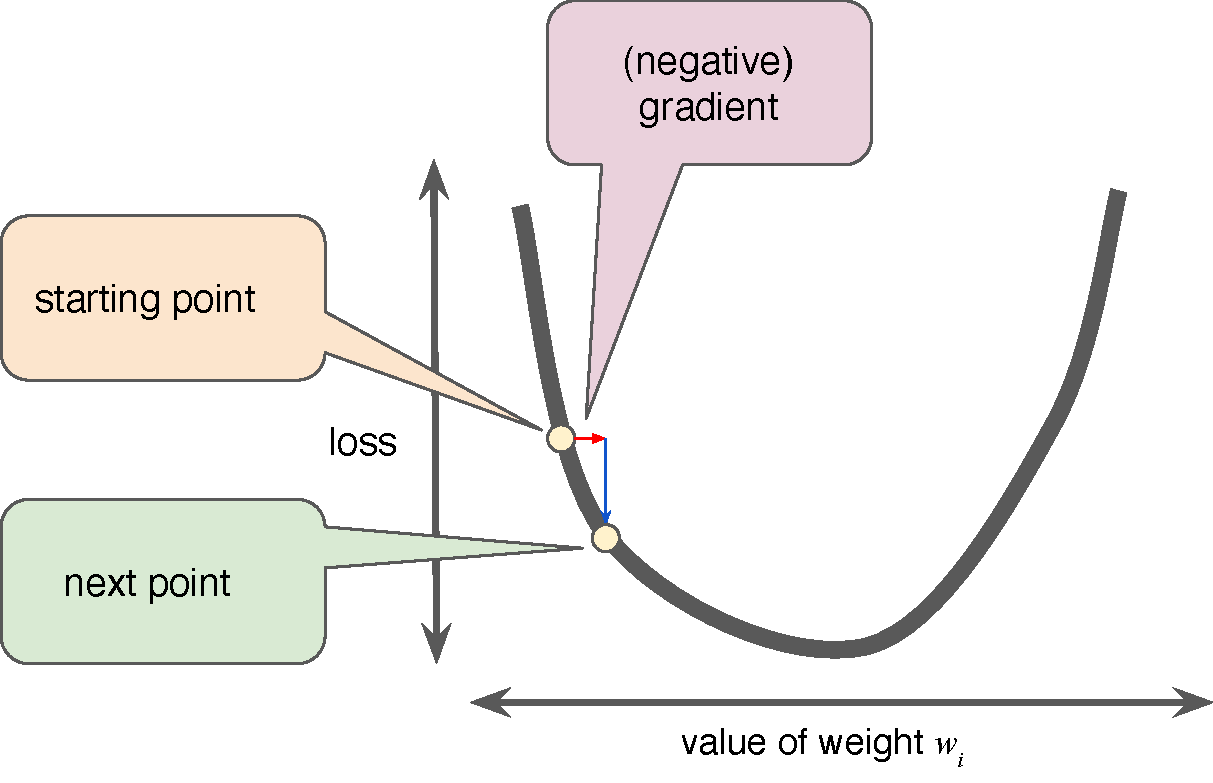
\includegraphics[width=0.5\linewidth]{images/supervised/training_reducing_loss/GradientDescentGradientStep.pdf}
			%\caption{Stripe Radar for Fraud Detection}
		\end{figure}
	%\end{block}

\end{frame}


\begin{frame}

	\frametitle{La discesa del gradiente}

	%\begin{block}{}
		Per determinare il punto successivo lungo la curva della loss, l'algoritmo di discesa del gradiente aggiunge una \textbf{frazione della intensità} del gradiente al punto iniziale come mostrato nella figura seguente:

		\begin{figure}[!htbp]
			\centering
			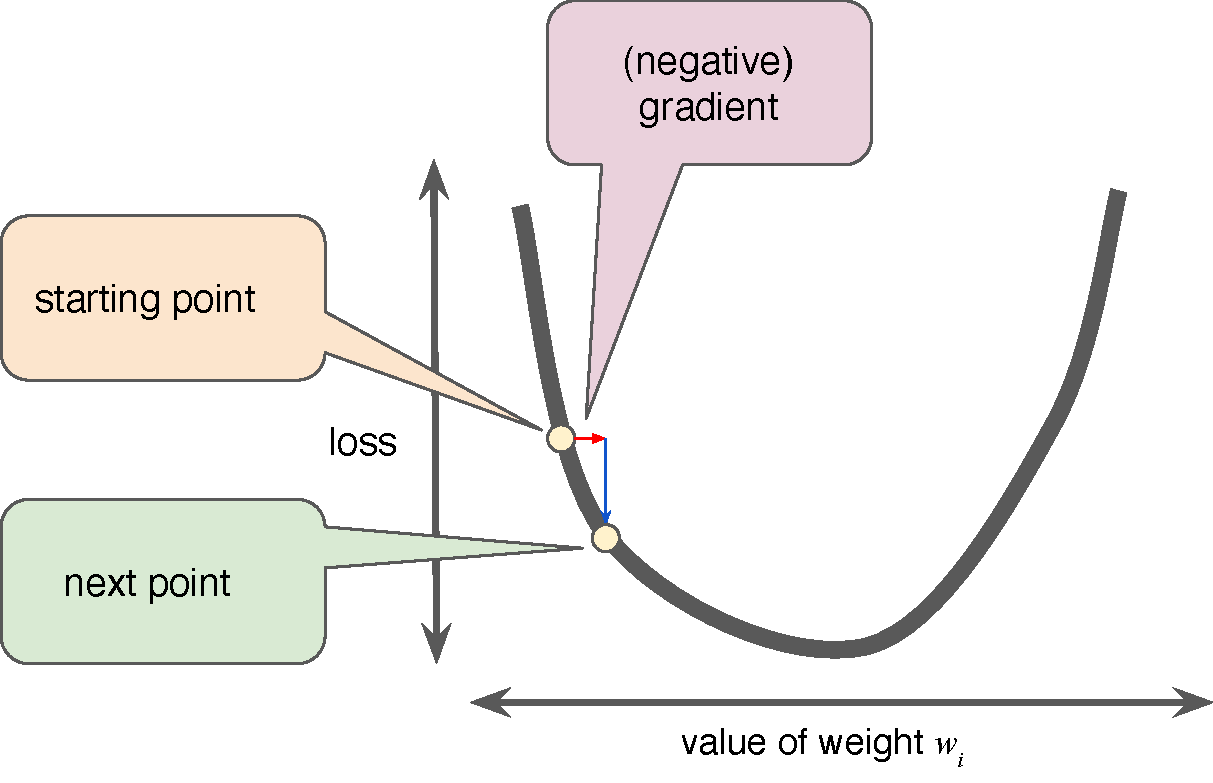
\includegraphics[width=0.5\linewidth]{images/supervised/training_reducing_loss/GradientDescentGradientStep.pdf}
			%\caption{Stripe Radar for Fraud Detection}
		\end{figure}

		La discesa del gradiente (GD) ripete quindi questo procedimento, avvicinandosi sempre più al minimo della funzione loss.
	%\end{block}

\end{frame}


\begin{frame}

	\frametitle{La discesa del gradiente}

	%\begin{block}{}
		\centering
		\animategraphics[controls={play, step, stop}, height=7cm]{1.0}{images/supervised/training_reducing_loss/gradient_descending/gd0/gradient_descending_0-}{0}{14}
	%\end{block}

\end{frame}


\begin{frame}

	\frametitle{La discesa del gradiente: il learning rate}

	\begin{block}{Il learning rate}
		Come notato, il vettore gradiente ha sia una direzione che una intensità.\\
		Gli algoritmi di discesa del gradiente moltiplicano il gradiente per uno scalare noto come \textbf{tasso di apprendimento} (\textbf{learning rate} o \textbf{step size}) per determinare il punto successivo.\\
		\vspace{3mm}
		Ad esempio, se l'ampiezza del gradiente è $2,5$ e il tasso di apprendimento è $0,01$, l'algoritmo di discesa del gradiente selezionerà il punto successivo $0,025$ dal punto precedente.\\
		\vspace{3mm}
		Valutiamo 3 casi:
		\begin{itemize}
			\item Un learning rate troppo piccolo
			\item Un learning rate troppo grande
			\item Un learning rate intermedio
		\end{itemize}
	\end{block}

\end{frame}



\begin{frame}

	\frametitle{La discesa del gradiente: il learning rate}

	\begin{block}{Un learning rate troppo piccolo}
		Se scegli un \textbf{learning rate troppo piccolo}, l'apprendimento richiederà troppo tempo:

		\begin{figure}[!htbp]
			\centering
			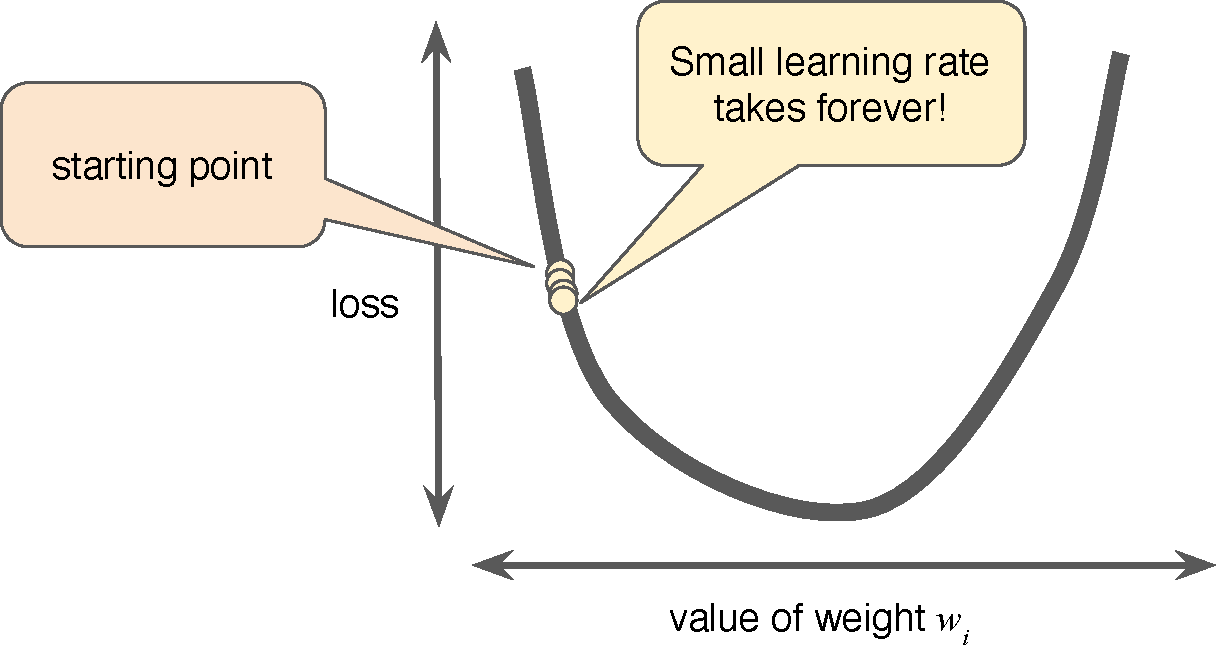
\includegraphics[height=0.4\linewidth]{images/supervised/training_reducing_loss/LearningRateTooSmall.pdf}
			%\caption{Stripe Radar for Fraud Detection}
		\end{figure}
	\end{block}

\end{frame}


\begin{frame}

	\frametitle{La discesa del gradiente: il learning rate}

	\begin{block}{Un learning rate troppo grande}
		Al contrario, se specifichi un \textbf{learning rate troppo grande}, il punto successivo rimbalzerà perennemente sul fondo della curva della loss:

		\begin{figure}[!htbp]
			\centering
			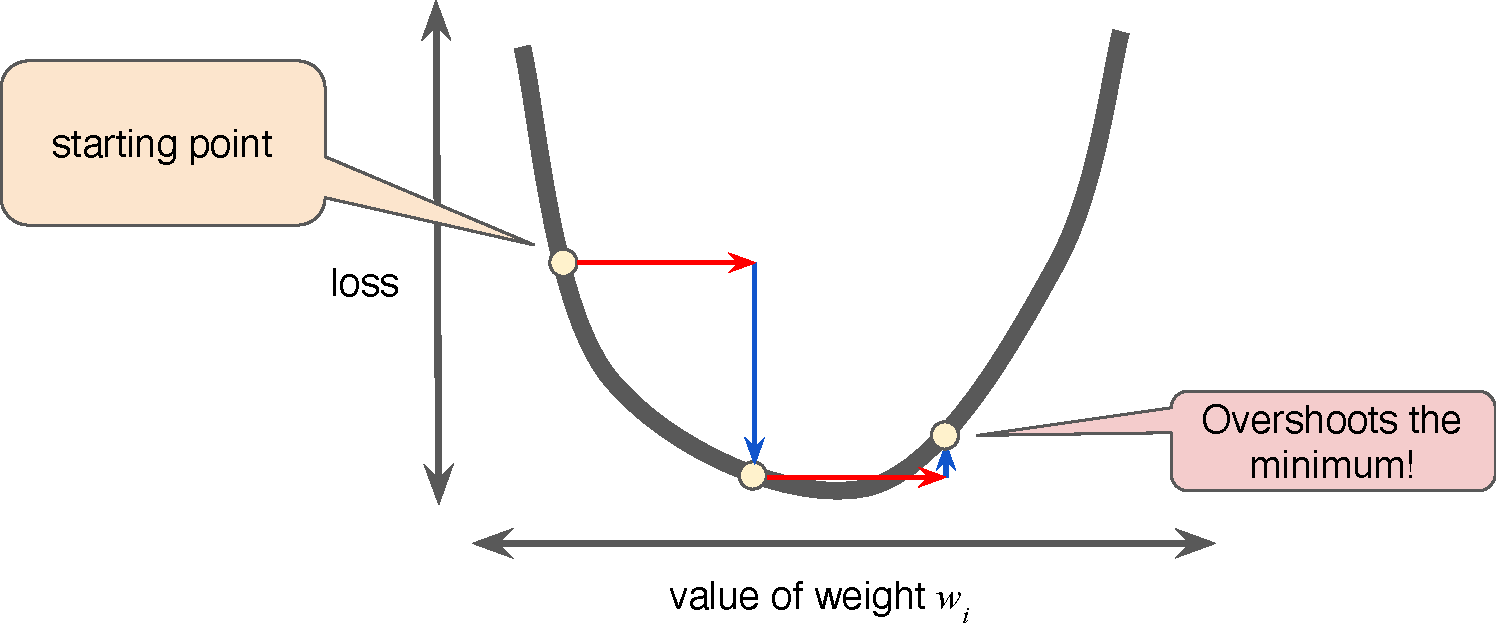
\includegraphics[height=0.4\linewidth]{images/supervised/training_reducing_loss/LearningRateTooLarge.pdf}
			%\caption{Stripe Radar for Fraud Detection}
		\end{figure}
	\end{block}

\end{frame}


\begin{frame}

	\frametitle{La discesa del gradiente: il learning rate}

	\begin{block}{Un learning rate intermedio}
		C'è un learning rate di \href{https://en.wikipedia.org/wiki/Goldilocks_principle}{Goldilocks} per ogni problema di regressione.\\
		Il valore di Goldilocks è correlato a quanto piatta è la funzione di perdita. Se sai che il gradiente della funzione di perdita è piccolo, puoi tranquillamente provare un tasso di apprendimento maggiore, che compensa il piccolo gradiente e si traduce in una dimensione del passo maggiore.

		\begin{figure}[!htbp]
			\centering
			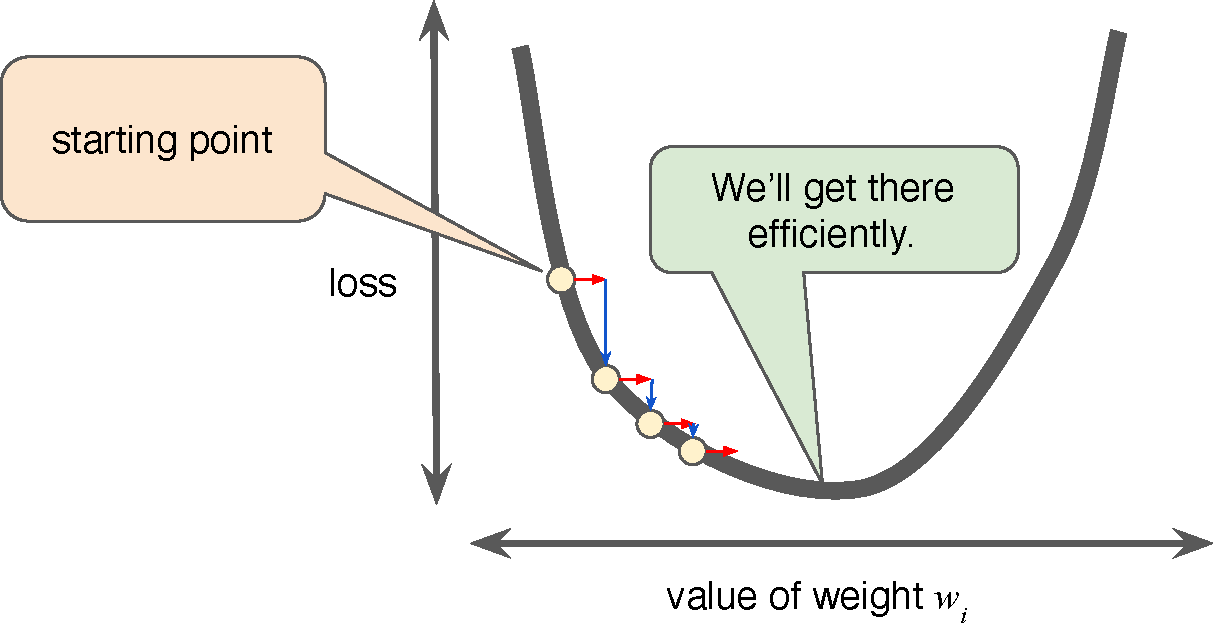
\includegraphics[height=0.25\linewidth]{images/supervised/training_reducing_loss/LearningRateJustRight.pdf}
			%\caption{Stripe Radar for Fraud Detection}
		\end{figure}
	\end{block}

\end{frame}


\begin{frame}

	\frametitle{La discesa del gradiente: il learning rate}

	%\begin{block}{}
		\centering
		\animategraphics[controls={play, step, stop}, height=7cm]{4.0}{images/supervised/training_reducing_loss/gradient_descending/gd1/gradient_descending_1-}{0}{25}
	%\end{block}

\end{frame}


\begin{frame}

	\frametitle{La discesa del gradiente}

	\begin{block}{Ricapitolando 1}
		L’algoritmo di \textbf{discesa del gradiente} è un perfetto esempio del funzionamento del machine learning e riassume in sé tutti i concetti espressi finora, perché è \textbf{comprensibile in modo intuitivo}, per immagini figurate, e non solamente attraverso le formule matematiche.
		\newlinedouble
		Inoltre, la discesa del gradiente, sebbene sia ben lungi dall’essere l’unico metodo possibile, è un approccio all’ottimizzazione ampiamente condiviso che viene \textbf{adottato da una serie di algoritmi di machine learning}, come i modelli lineari, le reti neurali e le macchine di gradient boosting.
	\end{block}

\end{frame}


\begin{frame}

	\frametitle{La discesa del gradiente}

	\begin{block}{Ricapitolando 2}
		Ragionando in modo figurato, il processo di ottimizzazione è un po’ come una \textbf{camminata in alta montagna in una giornata molto nebbiosa}: i parametri sono i diversi sentieri che si possono seguire per arrivare al fondovalle. A ogni passo avviene un’ottimizzazione della discesa del gradiente; a ogni iterazione, l’algoritmo sceglie il sentiero che riduce l’errore in maniera più consistente, indipendentemente dalla direzione precedentemente presa.
		\newlinedouble
		L’idea è che se i passi non sono troppo lunghi (il che porterebbe l’algoritmo a saltare a piè pari l’obiettivo), seguire sempre la direzione che scende di più porta alla fine a trovare il punto più basso. Purtroppo, questo non è sempre il risultato che si ottiene, perché \textbf{l’algoritmo può giungere a valli intermedie}, creando l’\textbf{illusione di aver raggiunto l’obiettivo}.
	\end{block}

\end{frame}


\begin{frame}

	\frametitle{La discesa del gradiente}

	\begin{block}{Ricapitolando 3}
		\begin{figure}[!htbp]
			\centering
			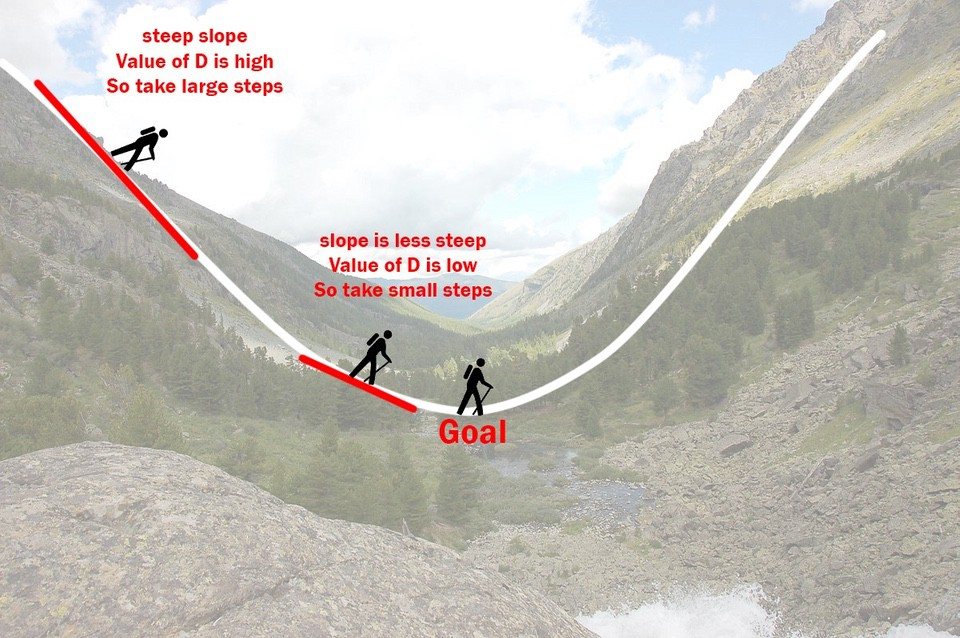
\includegraphics[height=6cm]{images/supervised/training_reducing_loss/gradient_descent_mountain_walk.jpeg}
			%\caption{Stripe Radar for Fraud Detection}
		\end{figure}

	\end{block}

\end{frame}


\begin{frame}

	\frametitle{La discesa del gradiente: esempio 1, modello $y=px$}

	%\begin{block}{}
		\centering
		\animategraphics[controls={play, step, stop}, height=5.0cm]{2.5}{images/supervised/training_reducing_loss/gradient_descending/gd2/gradient_descending_2-}{0}{11}
	%\end{block}

\end{frame}


\begin{frame}

	\frametitle{La discesa del gradiente: esempio 2, modello $y=b+mx$}

	%\begin{block}{}
		\centering
		\animategraphics[controls={play, step, stop}, height=4.25cm]{4}{images/supervised/training_reducing_loss/gradient_descending/gd3/gradient_descending_3-}{0}{19}
	%\end{block}

\end{frame}


\begin{frame}

	\frametitle{La discesa del gradiente: esempio 3, modello $y=b+mx$}

	%\begin{block}{}
		\centering
		\animategraphics[controls={play, step, stop}, height=5cm]{20.0}{images/supervised/training_reducing_loss/gradient_descending/gd4/gradient_descending_4-}{0}{80}
	%\end{block}

\end{frame}



\begin{frame}

	\frametitle{La discesa del gradiente: loss non convessa}

	\begin{block}{Una possibile soluzione nel caso di loss non convesse}
		In un processo di ottimizzazione, è necessario distinguere fra i diversi possibili esiti del processo. È possibile arrivare a un minimo globale, che rappresenta davvero l’errore minimo rispetto alla funzione di costo, ma è anche possibile giungere a svariati minimi locali, ossia soluzioni che sembrano produrre l’errore minimo, ma che in realtà non lo fanno – le vallate intermedie nelle quali l’algoritmo può rimanere bloccato.
		\newlinedouble
		Visto che \textbf{il processo di ottimizzazione inizia in maniera casuale, una buona soluzione consiste nel ripetere più volte l’ottimizzazione}: questo comporta provare diverse sequenze di sentieri in discesa, evitando il rischio di rimanere bloccati sempre nello stesso minimo locale.
	\end{block}

\end{frame}



\begin{frame}

	\frametitle{La discesa del gradiente: loss non convessa 1 (1 parametro)}

	%\begin{block}{}
		\begin{figure}[!htbp]
			\centering
			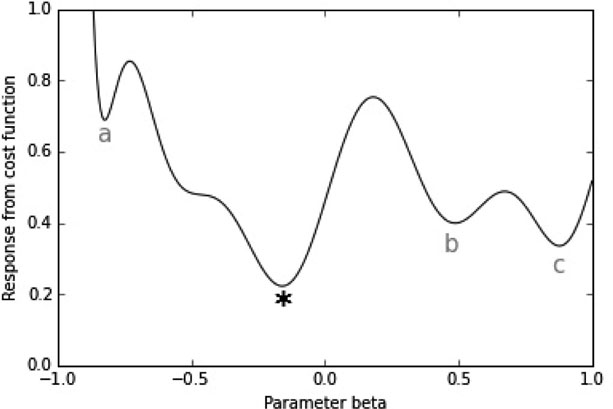
\includegraphics[width=10cm]{images/supervised/training_reducing_loss/non_convex_1.jpg}
			%\caption{Stripe Radar for Fraud Detection}
		\end{figure}

	%\end{block}

\end{frame}


\begin{frame}

	\frametitle{La discesa del gradiente: loss non convessa 2 (1 parametro)}
	%\begin{block}{}
		\centering
		\animategraphics[controls={play, step, stop}, height=7cm]{20.0}{images/supervised/training_reducing_loss/gradient_descending/gd5/gradient_descending_5-}{0}{199}
	%\end{block}

\end{frame}



\begin{frame}

	\frametitle{La discesa del gradiente: loss non convessa 3 (2 parametri)}

	%\begin{block}{}
		\begin{figure}[!htbp]
			\centering
			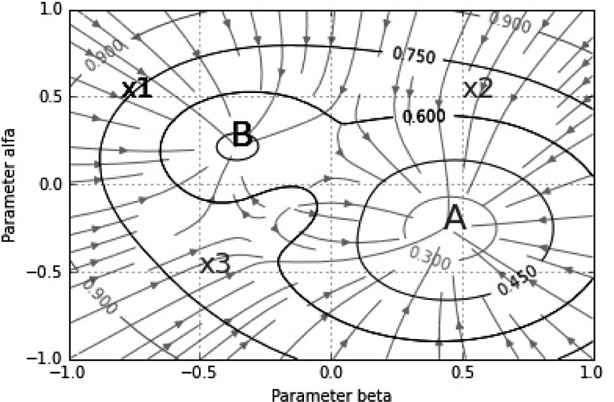
\includegraphics[width=10cm]{images/supervised/training_reducing_loss/non_convex_2.jpg}
			%\caption{Stripe Radar for Fraud Detection}
		\end{figure}

	%\end{block}

\end{frame}
